\documentclass[conference]{IEEEtran}

\usepackage{graphicx}
\usepackage{amsmath}
\usepackage{booktabs}
\usepackage{multirow}
\usepackage{url}
\usepackage[hidelinks]{hyperref}

\title{Image Dehazing using AOD-Net with Residual Learning and Skip Connections}

\author{
\IEEEauthorblockN{Ritwick Ranjan}
\IEEEauthorblockA{Department of Computer Science\\
Your Institute Name\\
Email: your.email@domain.com}
}

\begin{document}
\maketitle

\begin{abstract}
Image dehazing aims to recover clear scene content from images degraded by atmospheric scattering. This paper presents an academic project implementation of AOD-Net in a clean, modular workflow and studies two lightweight architectural extensions: residual learning and skip connections. The project is built from an existing PyTorch AOD-Net repository and refactored into a notebook-driven and web-based system suitable for presentation and experimentation. Using paired hazy and clean images from the RESIDE-6K dataset, we train baseline, residual, and skip-connection variants under a common setup. Experiments on a lightweight 600-pair subset show that the skip-connection model achieves the strongest saved-checkpoint validation PSNR of 19.65\,dB, while the baseline remains competitive with the lowest validation loss of 0.0163. In addition to the model study, the project delivers a polished Gradio-based interactive demo that allows users to upload hazy images, compare before-and-after views, and obtain dehazed results directly. The work demonstrates how a compact convolutional dehazing model can be transformed into a reproducible educational project with both analytical and practical value.
\end{abstract}

\begin{IEEEkeywords}
image dehazing, AOD-Net, residual learning, skip connections, convolutional neural network, RESIDE
\end{IEEEkeywords}

\section{Introduction}
Haze degrades image quality by reducing contrast, suppressing texture, and distorting scene visibility. These degradations affect not only human perception but also downstream computer vision tasks such as object detection, scene understanding, and autonomous navigation. Classical dehazing techniques often rely on priors such as the dark channel prior \cite{he2009darkchannel}. While effective in many cases, prior-driven methods can struggle when image statistics violate the assumptions encoded in the hand-crafted model.

Deep learning based dehazing methods reduce the need for manual feature design by learning a direct mapping from hazy images to clear outputs. Among lightweight CNN-based approaches, AOD-Net \cite{li2017aodnet} remains attractive because it is compact, fast, and easy to train. However, its simplicity also creates room for architectural exploration, especially when the goal is to preserve detail while keeping the system presentation-friendly for academic use.

This project addresses three objectives:
\begin{enumerate}
    \item reproduce the baseline AOD-Net pipeline in a modular and beginner-friendly form,
    \item evaluate residual and skip-connection variants under the same experimental setup, and
    \item extend the project into an interactive web application for practical image upload and inference.
\end{enumerate}

The overall article structure follows a clear research-writing progression centered on the problem statement, literature context, methodology, experimental evidence, and future scope. This organization is intended to keep the work focused, reproducible, and suitable for student presentation.

\section{Related Work}
Single image dehazing has been studied through both physical priors and learned models. The dark channel prior introduced by He \emph{et al.} \cite{he2009darkchannel} became one of the most influential classical methods by exploiting statistical regularities in haze-free images. Although powerful, prior-driven methods may produce artifacts in bright regions or complex atmospheric conditions.

CNN-based methods later reframed dehazing as a supervised image restoration task. DehazeNet \cite{cai2016dehazenet} demonstrated that an end-to-end convolutional design could estimate dehazing-related quantities directly from input images. AOD-Net \cite{li2017aodnet} further simplified the pipeline by integrating atmospheric modeling and restoration into one lightweight architecture. The RESIDE benchmark \cite{li2018reside} accelerated comparative work in this area by providing large-scale synthetic and real-world dehazing data resources.

Residual learning has become a standard deep learning tool after the success of ResNet \cite{he2016resnet}. In restoration problems, residual modeling can make optimization easier by asking the network to learn the corruption pattern rather than the full clean signal. Likewise, skip connections are often used to preserve low-level structures and spatial details. Motivated by these ideas, this project studies whether residual prediction and skip fusion can strengthen an otherwise lightweight AOD-Net-style model without turning the system into a heavy architecture.

\section{Methodology}
\subsection{Baseline AOD-Net}
The baseline model follows the compact AOD-Net spirit from the reference implementation. A small sequence of convolutional layers predicts a feature tensor \(k(x)\) from an input hazy image \(I(x)\). The restored image \(J(x)\) is then produced as
\begin{equation}
    J(x) = k(x)\cdot I(x) - k(x) + b,
\end{equation}
where \(b\) is a constant bias term. This formulation allows the network to internalize haze-related transformations while remaining computationally lightweight.

\subsection{Residual Learning Variant}
The residual variant predicts a haze residual \(R(x)\) and subtracts it from the input:
\begin{equation}
    \hat{J}(x) = I(x) - R(x).
\end{equation}
This design reduces the learning burden by encouraging the network to model the corruption component rather than reconstructing the entire clean image from scratch.

\subsection{Skip-Connection Variant}
The skip model keeps the learned restoration branch while introducing a learnable fusion path from the input image:
\begin{equation}
    \hat{J}(x) = F(I(x)) + \alpha \odot I(x),
\end{equation}
where \(F(\cdot)\) represents the convolutional restoration output and \(\alpha\) is a learnable channel-wise scaling factor. The intention is to preserve scene structure and texture while still allowing the network to correct haze-related distortions.

\subsection{Project Refactoring}
Beyond the models themselves, the repository was reorganized into four modular layers:
\begin{itemize}
    \item a notebook for step-by-step academic explanation,
    \item a reusable Python package for data, training, and inference,
    \item trained checkpoint files for all three variants, and
    \item a Gradio-based web interface for live demonstration.
\end{itemize}
The web interface was later refined with a cleaner layout, model-selection controls, a tabbed results workspace, a side-by-side preview panel, and live run details so that a user can dehaze uploaded images interactively during a classroom demonstration.

\section{Experimental Setup}
\subsection{Dataset}
The experiments use paired clean and hazy images from the RESIDE-6K dataset \cite{li2018reside}, downloaded through the Kaggle API. To keep the project lightweight and reproducible on modest hardware, training is performed on a 600-pair subset with an 80/20 train-validation split.

\subsection{Training Configuration}
All images are converted to RGB and resized to \(256 \times 256\). Each model is trained for 6 epochs with a batch size of 8 using the Adam optimizer. Mean Squared Error (MSE) is used as the training loss, and PSNR is used as the main image-quality metric. Table~\ref{tab:results} summarizes the saved-checkpoint results.

\begin{figure}[t]
    \centering
    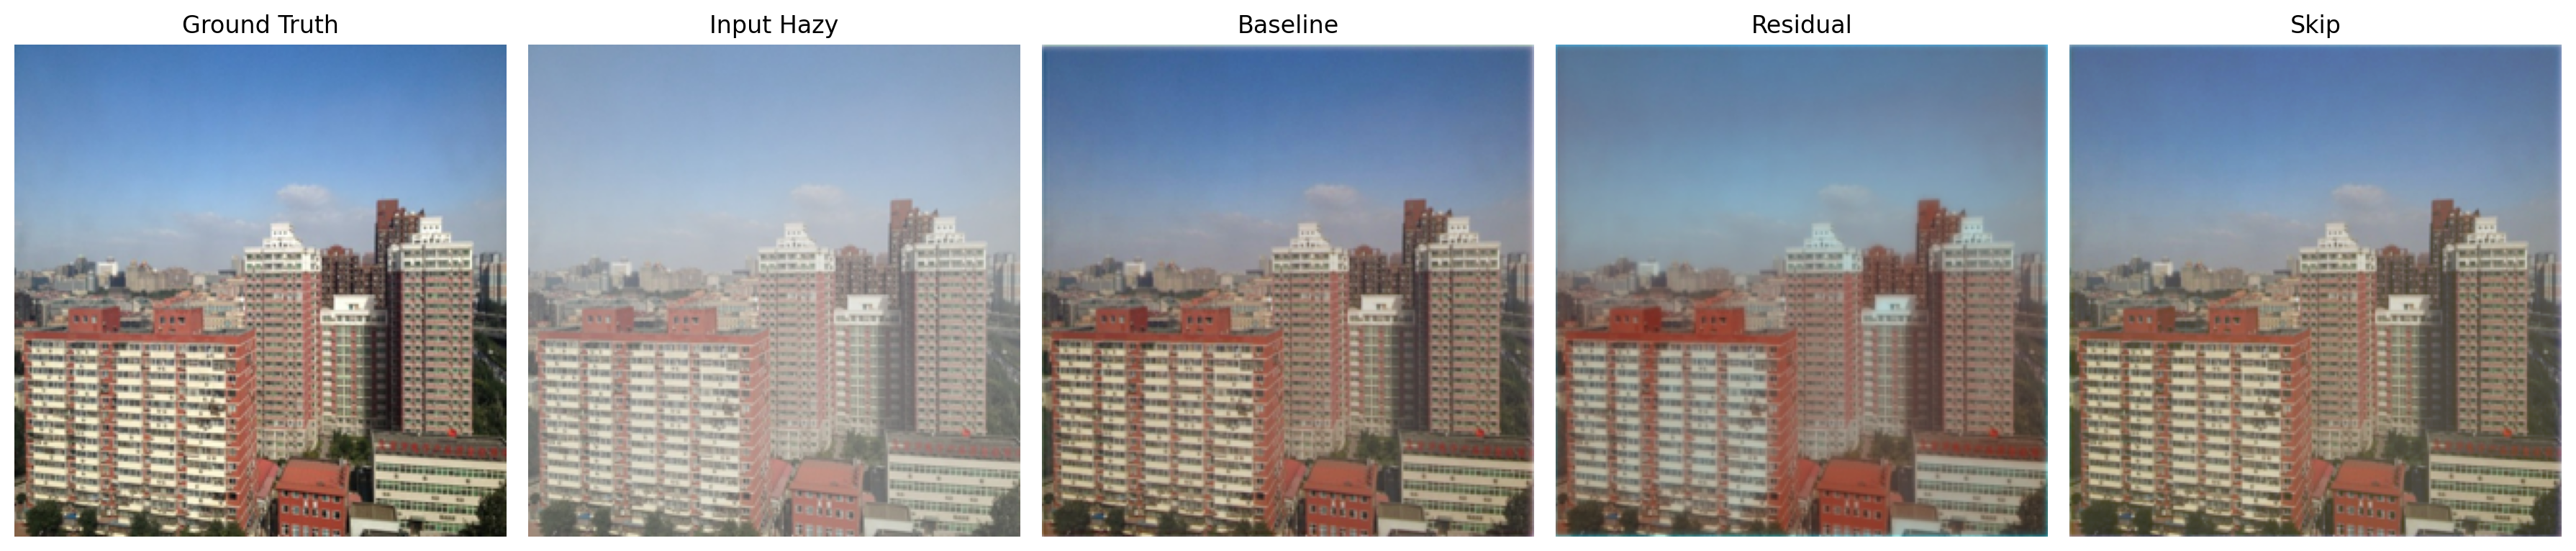
\includegraphics[width=\linewidth]{../assets/comparison_panel.png}
    \caption{Qualitative comparison on a sample RESIDE image. From left to right: ground truth, hazy input, baseline output, residual output, and skip-connection output.}
    \label{fig:qualitative}
\end{figure}

\section{Results and Discussion}
\subsection{Quantitative Results}
\begin{table}[t]
    \centering
    \caption{Validation results of the three trained variants.}
    \label{tab:results}
    \begin{tabular}{lccc}
        \toprule
        Model & Best Epoch & Val. Loss & Val. PSNR \\
        \midrule
        Baseline AOD-Net & 4 & 0.0163 & 19.50 \\
        Residual AOD-Net & 6 & 0.0177 & 18.89 \\
        Skip AOD-Net & 4 & 0.0163 & 19.65 \\
        \bottomrule
    \end{tabular}
\end{table}

The baseline and skip variants achieved almost identical validation loss, with the skip model slightly improving PSNR at the selected checkpoint. The residual variant remained stable and converged smoothly but did not outperform the other two under the current limited training budget. This suggests that residual reformulation alone may require longer training or additional regularization to fully benefit this lightweight setup.

\subsection{Training Dynamics}
Fig.~\ref{fig:curves} shows the validation loss and PSNR evolution across epochs. All three models improve rapidly during early training, which matches the expectation for a compact CNN operating on paired synthetic haze data. The skip-connection variant reaches the strongest peak PSNR trend, while the baseline remains the most consistent in terms of saved-checkpoint loss.

\begin{figure}[t]
    \centering
    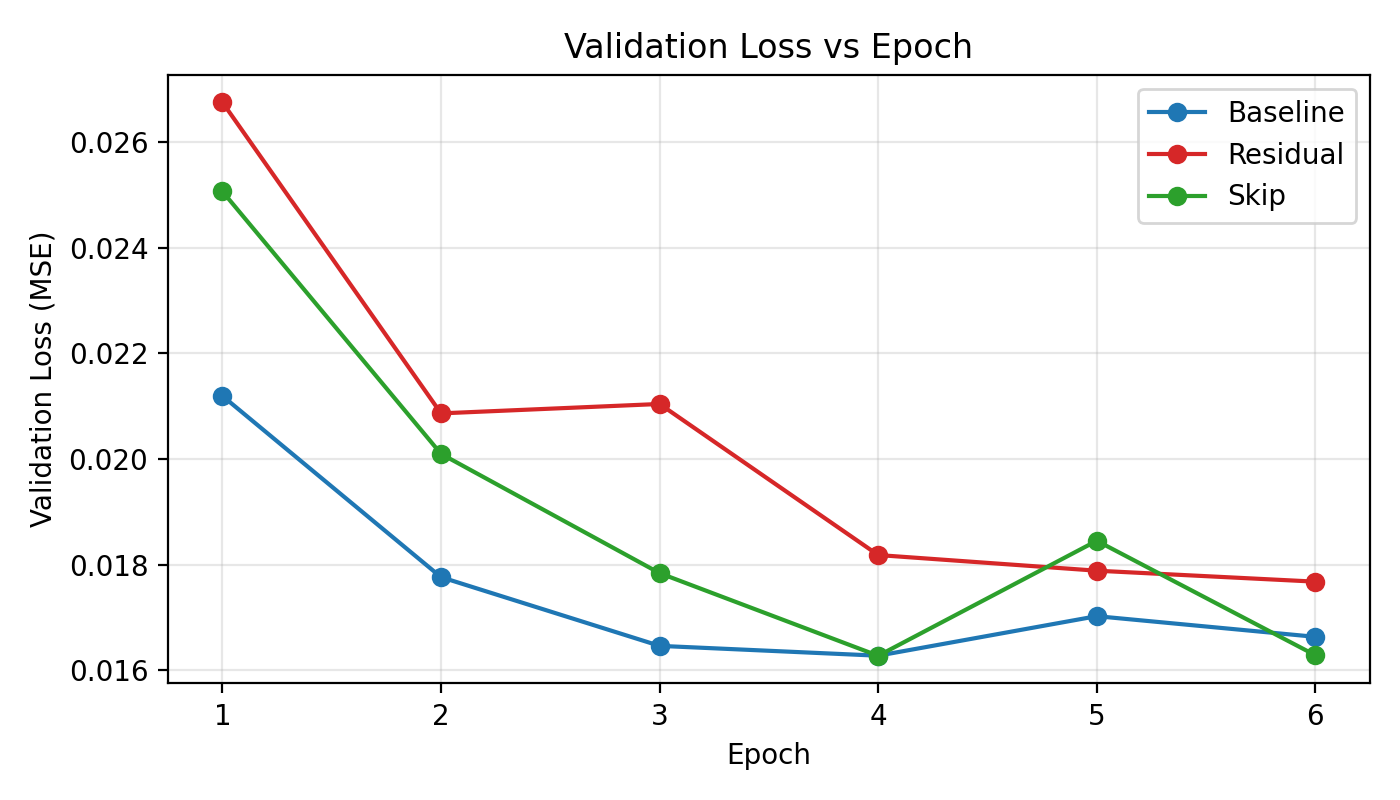
\includegraphics[width=\linewidth]{../assets/loss_curves.png}
    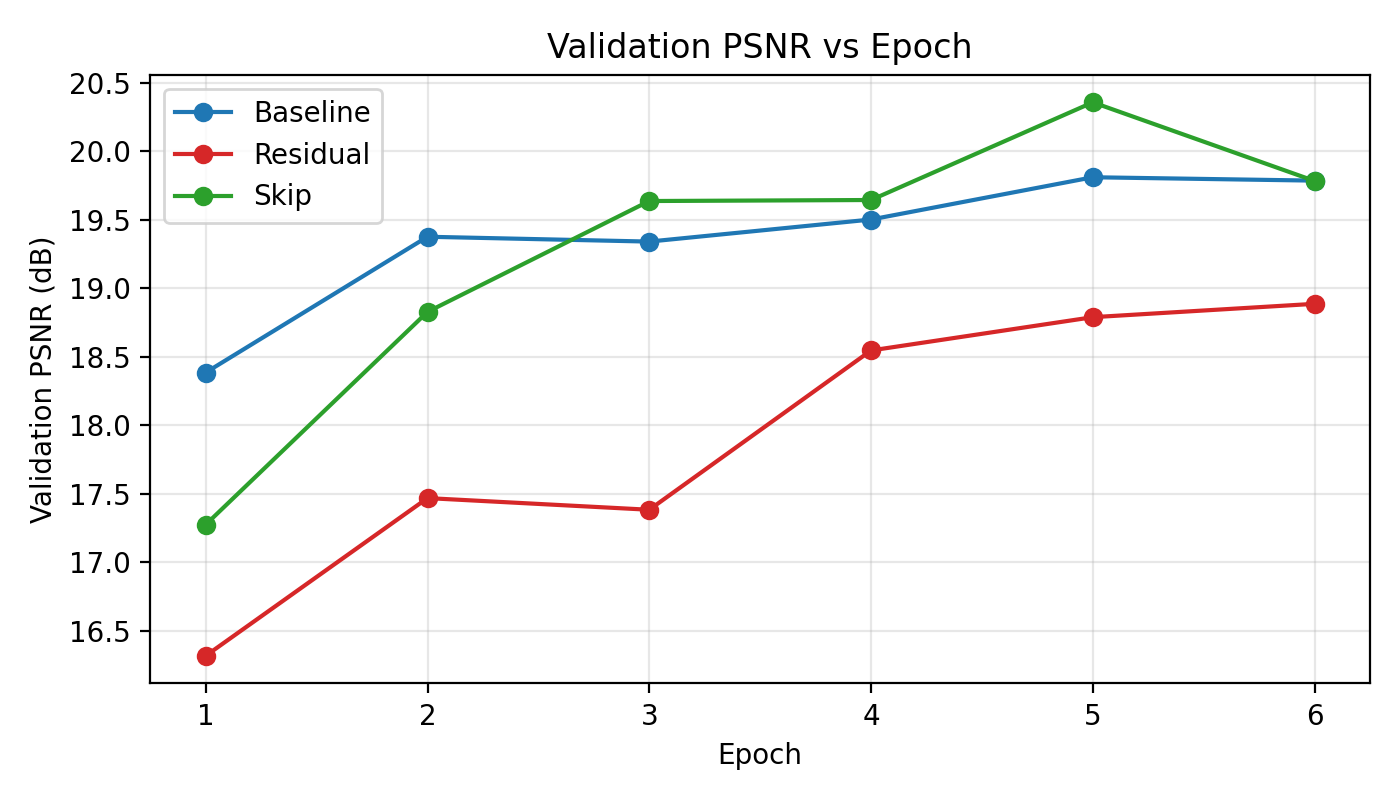
\includegraphics[width=\linewidth]{../assets/psnr_curves.png}
    \caption{Validation loss and PSNR curves across training epochs.}
    \label{fig:curves}
\end{figure}

\subsection{Qualitative Analysis}
Fig.~\ref{fig:qualitative} provides a representative visual comparison. All three models improve visibility compared with the hazy input. The skip-connection output retains scene structure more effectively in this sample, while the residual variant appears slightly softer. These observations are consistent with the idea that skip fusion helps preserve low-level image information.

\section{Interactive Web Demonstration}
To make the project presentation-ready, the trained models were deployed through a Gradio-based interface. The web system allows a user to upload a hazy image, select the baseline, residual, or skip model, and receive a dehazed result immediately. This extension makes the project useful not only as a model-comparison study but also as an interactive educational demonstration. Because the app reuses the same preprocessing and checkpoint pipeline as the notebook, its outputs remain consistent with the trained experiments.

The improved interface contains three practical features:
\begin{itemize}
    \item direct upload of a user image through the browser,
    \item model selection from the trained checkpoint set, and
    \item a tabbed result area with selected-model output, before-and-after view, and multi-model comparison.
\end{itemize}

Fig.~\ref{fig:webmockup} shows a representative interaction in which a user uploads a hazy outdoor image and receives the restored result from the skip-connection model. Fig.~\ref{fig:webpair} presents the uploaded image and the final dehazed output as a dedicated visual comparison panel. These figures emphasize that the project is not only a training notebook but also a usable application for image restoration.

\begin{figure*}[t]
    \centering
    
\includegraphics[width=\textwidth]{../assets/web_demo_mockup.png}
    \caption{Interactive web-based dehazing demo. A user uploads a hazy sample image on the left, runs the trained model, and receives the dehazed output on the right.}
    \label{fig:webmockup}
\end{figure*}

\begin{figure}[t]
    \centering
    
\includegraphics[width=\linewidth]{../assets/web_before_after_panel.png}
    \caption{Input-output view used in the web interface for quick visual inspection of the dehazing result.}
    \label{fig:webpair}
\end{figure}

\section{Conclusion and Future Scope}
This paper presented a modular academic implementation of image dehazing using AOD-Net and two lightweight extensions: residual learning and skip connections. The project reproduced the baseline AOD-Net workflow, organized it into a reusable notebook and web application, and evaluated all three variants on RESIDE image pairs. Under the current setup, the skip-connection model achieved the highest saved-checkpoint PSNR, while the baseline remained highly competitive in validation loss. The residual model offered a valid alternative formulation but would benefit from longer training and deeper tuning.

Future work will focus on full-dataset training, SSIM-based evaluation, stronger residual branch design, and richer web-based comparison tools for classroom demonstration.

\bibliographystyle{IEEEtran}
\bibliography{references}

\end{document}
